% Created by Bonita Graham
% Last update: February 2019 By Kestutis Bendinskas

% Authors: Breno de Castro Pimenta
% Please do not make changes to the preamble until after the solid line of %s.

\documentclass[10pt]{article}
\usepackage[explicit]{titlesec}
\setlength{\parindent}{0pt}
\setlength{\parskip}{1em}
\usepackage{hyphenat}
\usepackage{ragged2e}
\RaggedRight

% These commands change the font. If you do not have Garamond on your computer, you will need to install it.
\usepackage{garamondx}
\usepackage[T1]{fontenc}
\usepackage{amsmath, amsthm}
\usepackage{graphicx}

% This adjusts the underline to be in keeping with word processors.
\usepackage{soul}
\setul{.6pt}{.4pt}


% The following sets margins to 1 in. on top and bottom and .75 in on left and right, and remove page numbers.
\usepackage{geometry}
\geometry{vmargin={1in,1in}, hmargin={.75in, .75in}}
\usepackage{fancyhdr}
\pagestyle{fancy}
\pagenumbering{gobble}
\renewcommand{\headrulewidth}{0.0pt}
\renewcommand{\footrulewidth}{0.0pt}

% These Commands create the label style for tables, figures and equations.
\usepackage[labelfont={footnotesize,bf} , textfont=footnotesize]{caption}
\captionsetup{labelformat=simple, labelsep=period}
\newcommand\num{\addtocounter{equation}{1}\tag{\theequation}}
\renewcommand{\theequation}{\arabic{equation}}
\makeatletter
\renewcommand\tagform@[1]{\maketag@@@ {\ignorespaces {\footnotesize{\textbf{Equation}}} #1.\unskip \@@italiccorr }}
\makeatother
\setlength{\intextsep}{10pt}
\setlength{\abovecaptionskip}{2pt}
\setlength{\belowcaptionskip}{-10pt}

\renewcommand{\textfraction}{0.10}
\renewcommand{\topfraction}{0.85}
\renewcommand{\bottomfraction}{0.85}
\renewcommand{\floatpagefraction}{0.90}

% These commands set the paragraph and line spacing
\titleformat{\section}
  {\normalfont}{\thesection}{1em}{\MakeUppercase{\textbf{#1}}}
\titlespacing\section{0pt}{0pt}{-10pt}
\titleformat{\subsection}
  {\normalfont}{\thesubsection}{1em}{\textit{#1}}
\titlespacing\subsection{0pt}{0pt}{-8pt}
\renewcommand{\baselinestretch}{1.15}

% This designs the title display style for the maketitle command
\makeatletter
\newcommand\sixteen{\@setfontsize\sixteen{16pt}{6}}
\renewcommand{\maketitle}{\bgroup\setlength{\parindent}{0pt}
\begin{flushleft}
\vspace{-.375in}
\sixteen\bfseries \@title
\medskip
\end{flushleft}
\textit{\@author}
\egroup}
\makeatother

% This styles the bibliography and citations.
%\usepackage[biblabel]{cite}
\usepackage[sort&compress]{natbib}
\setlength\bibindent{2em}
\makeatletter
\renewcommand\@biblabel[1]{\textbf{#1.}\hfill}
\makeatother
\renewcommand{\citenumfont}[1]{\textbf{#1}}
\bibpunct{}{}{,~}{s}{,}{,}
\setlength{\bibsep}{0pt plus 0.3ex}




%%%%%%%%%%%%%%%%%%%%%%%%%%%%%%%%%%%%%%%%%%%%%%%%%

% Authors: Add additional packages and new commands here.  
% Limit your use of new commands and special formatting.

\title{Assignment  n$^{o}$ 2}

\author{
Breno de Castro Pimenta \\ \medskip 
RA: 2017114809 \\ \medskip \bigskip
DCC006: Computer Organization I  \\ 
Departamento de Ci{\^e}ncia da Computa{\c c}{\~a}o\\ 
Universidade Federal de Minas Gerais (UFMG) Brasil
\\ \medskip \bigskip}

\pagestyle{empty}
\begin{document}

% Makes the title and author information appear.
\vspace*{.01 in}
\maketitle
\vspace{.12 in}

\section*{Problem 1: 5-Stage Pipeline}
\medskip
O loop do programa descrito tarda nove ciclos de clock e {\'e} executado da seguinte forma: O loop se inicia com com o carregamento do pr{\'o}ximo valor do vetor (lw x12 0(x9)). Em seguida ele realiza um Add com depend{\^e}ncia do valor carregado na instru{\c c}{\~a}o anterior o que gera um Stall. Ap{\'o}s o Stall {\'e} realizado mais duas adi{\c c}{\~o}es. E no final para que o branch possa tomar a decis{\~a}o de continuar no loop ou continuar com as instru{\c c}{\~o}es normais, {\'e} realizado outros dois Stalls, pois o Branch necessita do valor calculado na instru{\c c}{\~a}o anterior. No pr{\'o}ximo ciclo ou a pr{\'o}xima instru{\c c}{\~a}o (fora do loop) que j{\'a} realizou o instruction fetch ser{\'a} realizada ou ser{\'a} ignorado seu instruction fetch e voltar{\'a} a executar outra itera{\c c}{\~a}o do loop.  A imagem abaixo demonstra o esquema gerado pelo simulador Ripes, com os ciclos enumerados.

\begin{figure}[ht!]
\centering
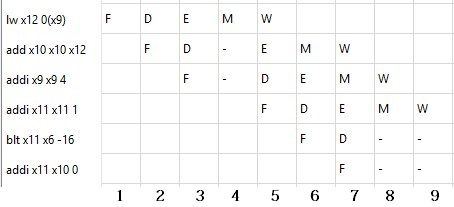
\includegraphics[width=0.65\textwidth]{CiclosLoopCount.jpg}
\caption{Diagrama de execu{\c c}{\~a}o do loop}\label{sample image}
\end{figure}

\vspace{.22 in}

\section*{Problem 2: Study Questions} 
\medskip
\medskip

\ul{Os cincos est{\'a}gios padr{\~o}es de um pipeline de um processador RISC:}\\\medskip
1. Fetch instruction: Busca a pr{\'o}xima instru{\c c}{\~a}o na mem{\'o}ria de instru{\c c}{\~o}es.\\
2. Instruction decode: Decodifica a instru{\c c}{\~a}o e l{\^e} do banco de registradores.\\
3. Execute: Executa opera{\c c}{\~o}es na ALU, desde opera{\c c}{\~o}es bin{\'a}rias, a aritm{\'e}ticas, at{\'e} c{\'a}lculo de endere{\c c}os.\\
4. Memory Access: Acessa a mem{\'o}ria principal para realizar escrita ou leitura (apenas parte das instru{\c c}{\~o}es realiza esse passo).\\
5. Write Back: Escreve resultados de opera{\c c}{\~o}es ou buscas no banco de registradores (apenas parte das instru{\c c}{\~o}es realiza esse passo).\\  \bigskip\bigskip\bigskip\bigskip\bigskip\bigskip\bigskip\bigskip\bigskip\bigskip\bigskip\bigskip\bigskip\bigskip\bigskip\bigskip\bigskip


\ul{Hazards:}\\
\medskip
Katz (1996) descreve Hazards como limita{\c c}{\~o}es do pipeline que previne  a pr{\'o}xima instru{\c c}{\~a}o de ser executada no tempo de clock designada a ela. 
\\\bigskip
\ul{Existem tr{\^e}s tipos de Hazards:}\\\bigskip
\ul{Hazard Estrutural:} \textbf{Defini{\c c}{\~a}o:} Quando uma instru{\c c}{\~a}o, devido ao conjunto de intru{\c c}{\~o}es que precedem ou sucedem essa instru{\c c}{\~a}o, a impedem de utilizar a estrutura de dados, ou seja de executar o procedimento que devia no ciclo de clock adequado. Sumariamente, s{\~a}o instru{\c c}{\~o}es tentando utilizar a mesma estrutura ao mesmo tempo.\\
\textbf{Exemplo:} Um exemplo para Hazard Estrutural {\'e} o levantado por Patterson e Hennessy (2018), onde {\'e} criado uma situa{\c c}{\~a}o hipot{\'e}tica onde s{\'o} haja uma estrutura de mem{\'o}ria no processador, e tenhamos uma instru{\c c}{\~a}o que acessa a mem{\'o}ria no quarto ciclo e esse ciclo {\'e} executado simult{\^a}neo a uma outra instru{\c c}{\~a}o que est{\'a} executando seu primeiro ciclo, buscando na mem{\'o}ria tamb{\'e}m, a tentativa de uso simultaneo da mesma estrutura no mesmo ciclo de clock gera ent{\~a}o o Hazard Estrutural. E nesse caso os pr{\'o}prios Patterson e Hennessy (2018) explicam que o conjunto de instru{\c c}{\~o}es do pipeline foi projetado para evitar esse tipo de instru{\c c}{\~o}es, tornando simples para os designers evitarem esse tipo de hazard, como no caso a cima que a utiliza{\c c}{\~a}o de duas mem{\'o}rias evita esse erro.\medskip

\ul{Hazard de Dados:} \textbf{Defini{\c c}{\~a}o}: Como esclarecido por Katz (1996) hazard de dados s{\~a}o causados por instru{\c c}{\~o}es, que para serem executadas, dependem de valores gerados por outras instru{\c c}{\~o}es que ainda est{\~a}o sendo processadas.\\
\textbf{Exemplo:} Um exemplo simples {\'e} a execu{\c c}{\~a}o de duas instru{\c c}{\~o}es do Tipo-R consecutivas, onde o resultado gerado na primeira {\'e} utilizado no processamento para gerar o resultado da segunda. Uma op{\c c}{\~a}o {\'e} deixar o compilador ordenar a execu{\c c}{\~a}o das instru{\c c}{\~o}es de forma a evitar a execu{\c c}{\~a}o sequencial de intru{\c c}{\~o}es interdependentes, por{\'e}m essas depend{\^e}ncias s{\~a}o muito frequentes e uma solu{\c c}{\~a}o simples para situa{\c c}{\~o}es como do caso apresentado a cima no exemplo, {\'e} a cria{\c c}{\~a}o de encaminhamentos. Encaminhamentos s{\~a}o a adi{\c c}{\~a}o de hardware (barramentos) de forma que permitam, assim que calculado o valor da instru{\c c}{\~a}o anterior, ele j{\'a} esteja dispon{\'i}vel para o uso na pr{\'o}xima instru{\c c}{\~a}o antes mesmo que ele esteja dispon{\'i}vel no banco de registradores ou na mem{\'o}ria. \medskip

\ul{Hazard de Controles:} \textbf{Defini{\c c}{\~a}o:} Centoducatte (1998) explica que hazard de controle, s{\~a}o problemas ocasionados pela execu{\c c}{\~a}o de instru{\c c}{\~o}es de desvio. Ou seja, quando uma instru{\c c}{\~a}o deve mudar o fluxo de execu{\c c}{\~a}o para outro ponto do c{\'o}digo, enquanto outras instru{\c c}{\~o}es sequenciais a ela j{\'a} come{\c c}aram a ser executadas.
\textbf{Exemplo:} O exemplo padr{\~a}o {\'e} uma instru{\c c}{\~a}o branch, que o tempo entre o processar o in{\'i}cio da instru{\c c}{\~a}o, executar a compara{\c c}{\~a}o e decida realizar o jump, toma quatro ciclos de clock. Nesse processo a instru{\c c}{\~a}o seguida ao branch j{\'a} ter{\'a} executado tamb{\'e}m tr{\^e}s ciclos, o que {\'e} um problema, pois caso o jump n{\~a}o for para a pr{\'o}xima instru{\c c}{\~a}o uma inconsit{\^e}ncia ter{\'a} sido gerada.Para solucionar esse tipo de problema {\'e} sempre necess{\'a}rio criar stalls ap{\'o}s o branch. Em casos normais 2 Stalls ser{\~a}o necess{\'a}rios para garantir a estabilidade do sistema, no entanto esse valor pode ser otimizado com a implementa{\c c}{\~a}o de um hardware auxiliar para tentar prever a a{\c c}{\~a}o do branch, antes mesmo de ser executado, o que em casos positivos economizaria 1 Stall ao processo.


\vspace{2.4 in}


\section*{Problem 3: Exercise 4.22 reproduced from the textbook}

\bigskip

\textbf{3.1)} O diagrama abaixo demonstra onde ir{\'a} acontecer os dois hazard estruturais caso o fragmento de c{\'o}digo fosse executado sem a adi{\c c}{\~a}o dos Stalls.

\begin{figure}[ht!]
\centering
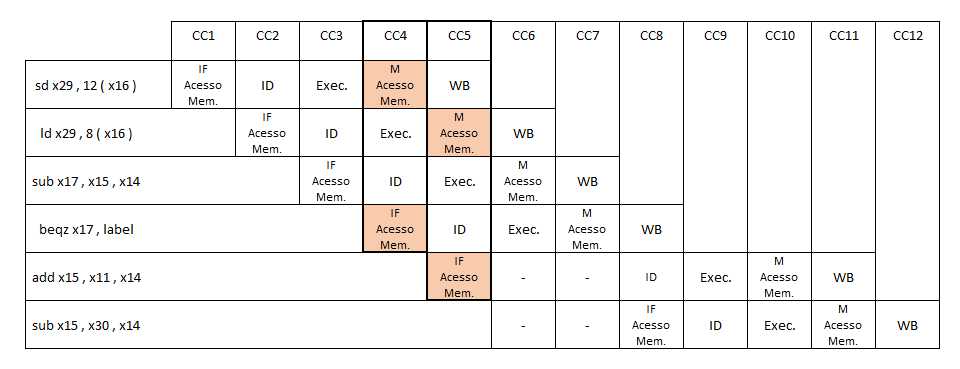
\includegraphics[width=0.65\textwidth]{Diagrama_pipeLine.png}
\caption{Diagrama de localiza{\c c}{\~a}o dos ciclos onde devem ser realizados os Stall{\'}s}\label{sample image}
\end{figure}

\bigskip
\bigskip
O primeiro Stall {\'e} no quarto ciclo, quando o store tenta escrever na mem{\'o}ria ao mesmo tempo que o branch tenta ler a instru{\c c}{\~a}o tamb{\'e}m na mem{\'o}ria.
O segundo Stall deve acontecer no quinto ciclo, onde o load tenta acessar a mem{\'o}ria, enquanto ao mesmo tempo o comando add tenta buscar na mesma mem{\'o}ria sua instru{\c c}{\~a}o.
Para resolver isso deve ser executado um Stall em ambos os ciclos mencionados a cima resultando no seguinte diagrama.\\\bigskip \bigskip

\begin{figure}[ht!]
\centering
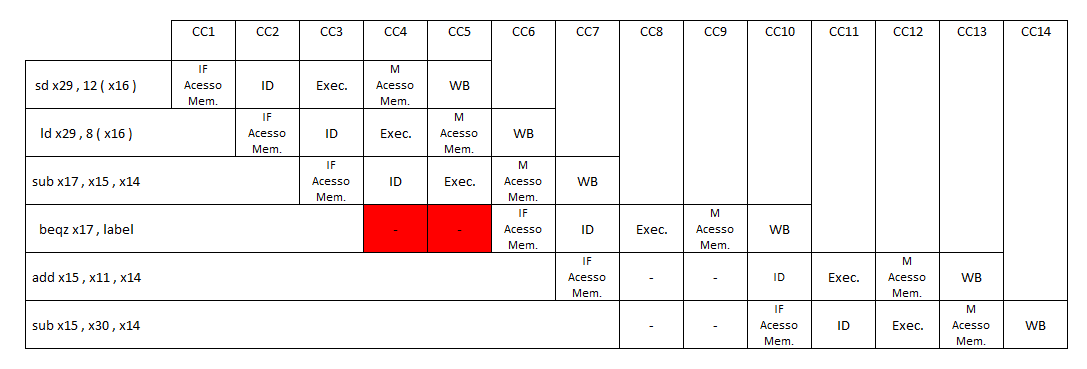
\includegraphics[width=0.80\textwidth]{Diagrama_pipeLine_Stalls.png}
\caption{Diagrama com os Stall's}\label{sample image}
\end{figure}

\bigskip
\bigskip
\textbf{3.2)} H{\'a} como reorganizar as instru{\c c}{\~o}es para ter um ganho com a diminui{\c c}{\~a}o de Stalls.
Partindo do princ{\'i}pio que as instru{\c c}{\~o}es que precedem o branch n{\~a}o podem ser realocadas para depois do branch, pois o branch pode pular para outro lugar e as instru{\c c}{\~o}es que o precedem j{\'a} devem ter sido executadas enquanto as que o sucedem devem. 
Logo o inverso tamb{\'e}m {\'e} verdadeiro, n{\~a}o se pode trocar as instru{\c c}{\~o}es que sucedem com as que precedem o branch. Com isso dito, temos dois blocos que podem ser reorganizados, no entanto as intru{\c c}{\~o}es que sucedem o branch, tanto n{\~a}o geram ganho em rela{\c c}{\~a}o a Stalls, como n{\~a}o podem ser trocadas devido a deped{\^e}ncias.
J{\'a} detre as intru{\c c}{\~o}es que precedem o Branch n{\~a}o se pode trocar o load com o store, entre si, j{\'a} que o valor que o strore armazena pode ser diferente do que o load est{\'a} carregando. Finalmente resta apenas uma op{\c c}{\~a}o, movimentar a instru{\c c}{\~a}o \textbf{sub} que precede o branch, ou para o in{\'i}cio das instru{\c c}{\~o}es load e store ou para entre elas. Em ambos os casos anteriores, ao mover-se a instru{\c c}{\~a}o \textbf{sub}, o fragmento de c{\'o}digo ter{\'a} o ganho de um Stall, pois o load ser{\'a} executado logo antes do Branch, o que acarretar{\'a} ao acesso {\'a} mem{\'o}ria do load, do seu quarto ciclo, seja executado juntamente com um Stall do branch, como pode ser visto no diagrama abaixo em verde.\\\bigskip\bigskip

\begin{figure}[ht!]
\centering
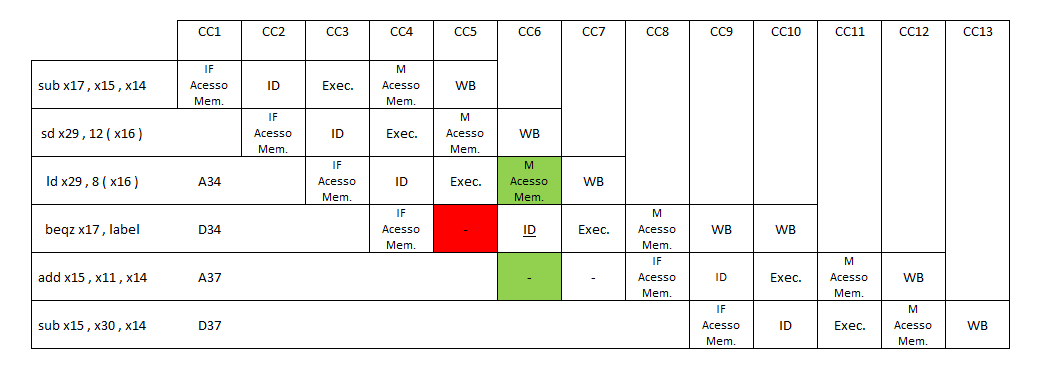
\includegraphics[width=0.80\textwidth]{Diagrama_reorganizacao.png}
\caption{Diagrama com a reorganiza{\c c}{\~a}o do c{\'o}digo, gerando a economia de um Stall}\label{sample image}
\end{figure}

\bigskip
\bigskip
\textbf{3.3)}  O Hazard de Dados enfrenta um problema de localiza{\c c}{\~a}o espacial de dados j{\'a} processados, neste caso a adi{\c c}{\~a}o de barramentos, tamb{\'e}m conhecido como encaminhamento, soluciona o problema, pois o simples acesso a um dado em uma posi{\c c}{\~a}o diferente soluciona o problema. 
Diferentemente do anterior, o Hazard estrutural enfrenta um problema de processamento de dados, pois ele exige dois processamentos distintos de uma mesma estrutura de dados no mesmo ciclo de clock. A simples adi{\c c}{\~a}o de barramento para melhorar a disposi{\c c}{\~a}o espacial dos dados n{\~a}o faz diferen{\c c}a para a realiza{\c c}{\~a}o dessa tarefa. A {\'u}nica solu{\c c}{\~a}o {\'e} adicionar outras estruturas de dados ao data path e apontar cada instru{\c c}{\~a}o para uma estrutura diferente, de forma a realizar ambos os processamentos em paralelo e ao final do ciclo ter processado ambos os dados. Outra op{\c c}ao {\'e} trocar a estrutura de dados em quest{\~a}o por uma mais avan{\c c}ada que permita processamento em paralelo em um {\'u}nico ciclo (caso exista).

\vspace{0.6 in}

\begin{thebibliography}{9} 

\bibitem{journal} CENTODUCATTE, P. C. \textbf{Pipeline}. Morgan Kaufmann Publishers. Unicamp. Campinas, S{\~a}o Paulo, Brasil, 1998. \textit {http://www.ic.unicamp.br/~pannain/mc722/aulas/arq_hp6.pdf}

\bibitem{journal}KATZ, R. H. \textbf{Lecture 7}: Introduction to Pipelining, Structural Hazards, and Forwarding. Berkeley, CA, Estados Unidos, 1996.   \textit{http://bnrg.cs.berkeley.edu/~randy/Courses/CS252.S96/Lecture07.pdf}\\

\bibitem{journal}PATTERSO, D. A.; HENNESSY J. L. \textbf{Computer Organization and Design:} THE HARDWARE/SOFTWARE INTERFACE. RiscV Edition. Morgan Kaufmann. Cambridge, MA, Estados Unidos, 2018.  \textit {https://www.academia.edu/38301807/Computer_organization_and_design_RISC_V}
\end{thebibliography}

\end{document}
